% Options for packages loaded elsewhere
\PassOptionsToPackage{unicode}{hyperref}
\PassOptionsToPackage{hyphens}{url}
\documentclass[
  man,mask]{apa6}
\usepackage{xcolor}
\usepackage{amsmath,amssymb}
\setcounter{secnumdepth}{-\maxdimen} % remove section numbering
\usepackage{iftex}
\ifPDFTeX
  \usepackage[T1]{fontenc}
  \usepackage[utf8]{inputenc}
  \usepackage{textcomp} % provide euro and other symbols
\else % if luatex or xetex
  \usepackage{unicode-math} % this also loads fontspec
  \defaultfontfeatures{Scale=MatchLowercase}
  \defaultfontfeatures[\rmfamily]{Ligatures=TeX,Scale=1}
\fi
\usepackage{lmodern}
\ifPDFTeX\else
  % xetex/luatex font selection
\fi
% Use upquote if available, for straight quotes in verbatim environments
\IfFileExists{upquote.sty}{\usepackage{upquote}}{}
\IfFileExists{microtype.sty}{% use microtype if available
  \usepackage[]{microtype}
  \UseMicrotypeSet[protrusion]{basicmath} % disable protrusion for tt fonts
}{}
\makeatletter
\@ifundefined{KOMAClassName}{% if non-KOMA class
  \IfFileExists{parskip.sty}{%
    \usepackage{parskip}
  }{% else
    \setlength{\parindent}{0pt}
    \setlength{\parskip}{6pt plus 2pt minus 1pt}}
}{% if KOMA class
  \KOMAoptions{parskip=half}}
\makeatother
% Make \paragraph and \subparagraph free-standing
\makeatletter
\ifx\paragraph\undefined\else
  \let\oldparagraph\paragraph
  \renewcommand{\paragraph}{
    \@ifstar
      \xxxParagraphStar
      \xxxParagraphNoStar
  }
  \newcommand{\xxxParagraphStar}[1]{\oldparagraph*{#1}\mbox{}}
  \newcommand{\xxxParagraphNoStar}[1]{\oldparagraph{#1}\mbox{}}
\fi
\ifx\subparagraph\undefined\else
  \let\oldsubparagraph\subparagraph
  \renewcommand{\subparagraph}{
    \@ifstar
      \xxxSubParagraphStar
      \xxxSubParagraphNoStar
  }
  \newcommand{\xxxSubParagraphStar}[1]{\oldsubparagraph*{#1}\mbox{}}
  \newcommand{\xxxSubParagraphNoStar}[1]{\oldsubparagraph{#1}\mbox{}}
\fi
\makeatother
\usepackage{graphicx}
\makeatletter
\newsavebox\pandoc@box
\newcommand*\pandocbounded[1]{% scales image to fit in text height/width
  \sbox\pandoc@box{#1}%
  \Gscale@div\@tempa{\textheight}{\dimexpr\ht\pandoc@box+\dp\pandoc@box\relax}%
  \Gscale@div\@tempb{\linewidth}{\wd\pandoc@box}%
  \ifdim\@tempb\p@<\@tempa\p@\let\@tempa\@tempb\fi% select the smaller of both
  \ifdim\@tempa\p@<\p@\scalebox{\@tempa}{\usebox\pandoc@box}%
  \else\usebox{\pandoc@box}%
  \fi%
}
% Set default figure placement to htbp
\def\fps@figure{htbp}
\makeatother
% definitions for citeproc citations
\NewDocumentCommand\citeproctext{}{}
\NewDocumentCommand\citeproc{mm}{%
  \begingroup\def\citeproctext{#2}\cite{#1}\endgroup}
\makeatletter
 % allow citations to break across lines
 \let\@cite@ofmt\@firstofone
 % avoid brackets around text for \cite:
 \def\@biblabel#1{}
 \def\@cite#1#2{{#1\if@tempswa , #2\fi}}
\makeatother
\newlength{\cslhangindent}
\setlength{\cslhangindent}{1.5em}
\newlength{\csllabelwidth}
\setlength{\csllabelwidth}{3em}
\newenvironment{CSLReferences}[2] % #1 hanging-indent, #2 entry-spacing
 {\begin{list}{}{%
  \setlength{\itemindent}{0pt}
  \setlength{\leftmargin}{0pt}
  \setlength{\parsep}{0pt}
  % turn on hanging indent if param 1 is 1
  \ifodd #1
   \setlength{\leftmargin}{\cslhangindent}
   \setlength{\itemindent}{-1\cslhangindent}
  \fi
  % set entry spacing
  \setlength{\itemsep}{#2\baselineskip}}}
 {\end{list}}
\usepackage{calc}
\newcommand{\CSLBlock}[1]{\hfill\break\parbox[t]{\linewidth}{\strut\ignorespaces#1\strut}}
\newcommand{\CSLLeftMargin}[1]{\parbox[t]{\csllabelwidth}{\strut#1\strut}}
\newcommand{\CSLRightInline}[1]{\parbox[t]{\linewidth - \csllabelwidth}{\strut#1\strut}}
\newcommand{\CSLIndent}[1]{\hspace{\cslhangindent}#1}
\ifLuaTeX
\usepackage[bidi=basic]{babel}
\else
\usepackage[bidi=default]{babel}
\fi
\babelprovide[main,import]{english}
% get rid of language-specific shorthands (see #6817):
\let\LanguageShortHands\languageshorthands
\def\languageshorthands#1{}
\ifLuaTeX
  \usepackage[english]{selnolig} % disable illegal ligatures
\fi
\setlength{\emergencystretch}{3em} % prevent overfull lines
\providecommand{\tightlist}{%
  \setlength{\itemsep}{0pt}\setlength{\parskip}{0pt}}
% Manuscript styling
\usepackage{upgreek}
\captionsetup{font=singlespacing,justification=justified}

% Table formatting
\usepackage{longtable}
\usepackage{lscape}
% \usepackage[counterclockwise]{rotating}   % Landscape page setup for large tables
\usepackage{multirow}		% Table styling
\usepackage{tabularx}		% Control Column width
\usepackage[flushleft]{threeparttable}	% Allows for three part tables with a specified notes section
\usepackage{threeparttablex}            % Lets threeparttable work with longtable

% Create new environments so endfloat can handle them
% \newenvironment{ltable}
%   {\begin{landscape}\centering\begin{threeparttable}}
%   {\end{threeparttable}\end{landscape}}
\newenvironment{lltable}{\begin{landscape}\centering\begin{ThreePartTable}}{\end{ThreePartTable}\end{landscape}}

% Enables adjusting longtable caption width to table width
% Solution found at http://golatex.de/longtable-mit-caption-so-breit-wie-die-tabelle-t15767.html
\makeatletter
\newcommand\LastLTentrywidth{1em}
\newlength\longtablewidth
\setlength{\longtablewidth}{1in}
\newcommand{\getlongtablewidth}{\begingroup \ifcsname LT@\roman{LT@tables}\endcsname \global\longtablewidth=0pt \renewcommand{\LT@entry}[2]{\global\advance\longtablewidth by ##2\relax\gdef\LastLTentrywidth{##2}}\@nameuse{LT@\roman{LT@tables}} \fi \endgroup}

% \setlength{\parindent}{0.5in}
% \setlength{\parskip}{0pt plus 0pt minus 0pt}

% Overwrite redefinition of paragraph and subparagraph by the default LaTeX template
% See https://github.com/crsh/papaja/issues/292
\makeatletter
\renewcommand{\paragraph}{\@startsection{paragraph}{4}{\parindent}%
  {0\baselineskip \@plus 0.2ex \@minus 0.2ex}%
  {-1em}%
  {\normalfont\normalsize\bfseries\itshape\typesectitle}}

\renewcommand{\subparagraph}[1]{\@startsection{subparagraph}{5}{1em}%
  {0\baselineskip \@plus 0.2ex \@minus 0.2ex}%
  {-\z@\relax}%
  {\normalfont\normalsize\itshape\hspace{\parindent}{#1}\textit{\addperi}}{\relax}}
\makeatother

\makeatletter
\usepackage{etoolbox}
\patchcmd{\maketitle}
  {\section{\normalfont\normalsize\abstractname}}
  {\section*{\normalfont\normalsize\abstractname}}
  {}{\typeout{Failed to patch abstract.}}
\patchcmd{\maketitle}
  {\section{\protect\normalfont{\@title}}}
  {\section*{\protect\normalfont{\@title}}}
  {}{\typeout{Failed to patch title.}}
\makeatother

\usepackage{xpatch}
\makeatletter
\xapptocmd\appendix
  {\xapptocmd\section
    {\addcontentsline{toc}{section}{\appendixname\ifoneappendix\else~\theappendix\fi\\: #1}}
    {}{\InnerPatchFailed}%
  }
{}{\PatchFailed}
\keywords{visual concepts, receptive vocabulary, large language models, object recognition\newline\indent Word count: 1486 excluding Method/Results}
\DeclareDelayedFloatFlavor{ThreePartTable}{table}
\DeclareDelayedFloatFlavor{lltable}{table}
\DeclareDelayedFloatFlavor*{longtable}{table}
\makeatletter
\renewcommand{\efloat@iwrite}[1]{\immediate\expandafter\protected@write\csname efloat@post#1\endcsname{}}
\makeatother
\usepackage{lineno}

\linenumbers
\usepackage{csquotes}
\usepackage[titles]{tocloft}
\cftpagenumbersoff{figure}
\renewcommand{\cftfigpresnum}{\itshape\figurename\enspace}
\renewcommand{\cftfigaftersnum}{.\space}
\setlength{\cftfigindent}{0pt}
\setlength{\cftafterloftitleskip}{0pt}
\settowidth{\cftfignumwidth}{Figure 10.\qquad}
\usepackage{bookmark}
\IfFileExists{xurl.sty}{\usepackage{xurl}}{} % add URL line breaks if available
\urlstyle{same}
\hypersetup{
  pdftitle={Developmental changes in the precision of visual concept knowledge},
  pdflang={en-EN},
  pdfkeywords={visual concepts, receptive vocabulary, large language models, object recognition},
  hidelinks,
  pdfcreator={LaTeX via pandoc}}

\title{Developmental changes in the precision of visual concept knowledge}
\author{Bria Long\textsuperscript{1}, Wanjing Anya Ma\textsuperscript{2}, Alvin W. M. Tan\textsuperscript{2}, Rebecca Silverman\textsuperscript{2}, Jason D. Yeatmean\textsuperscript{2}, \& Michael C. Frank\textsuperscript{2}}
\date{}


\shorttitle{Precision of visual concepts}

\authornote{

.

Correspondence concerning this article should be addressed to Bria Long. E-mail: \href{mailto:brlong@ucsd.edu}{\nolinkurl{brlong@ucsd.edu}}

}

\affiliation{\vspace{0.5cm}\textsuperscript{1} University of California San Diego\\\textsuperscript{2} Stanford University}

\abstract{%
How precise is children's visual concept knowledge, and how does this change across development? We created a gamified picture-matching task where children heard a word (e.g., ``swordfish'') and had to choose the picture ``that goes with the word.'' We collected data from large sample of children on this task (N = 3467, 3-14 years of age) and adults (N = 211), and we modeled changes in the proportion of children who chose a given image for a certain word over this developmental age range. We found gradual changes across this age range in children's ability to identify the correct category, highlighting a protracted developmental trajectory. Error analysis revealed that children were more likely to choose higher-similarity distractors as they grew older; further, children's error patterns were increasingly correlated with target-distractor similarity in the linguistic and multimodal embedding spaces of a large multimodal language model. These analyses suggest a transition from coarse to finer-grained visual representations over early and middle childhood, while emphasizing that even young children have partial knowledge for many difficult visual concepts. More broadly, these findings demonstrate the utility of combining gamified experiments and similarity estimates from computational models to probe the content of children's evolving visual representations.
}



\begin{document}
\maketitle

\section{Introduction}\label{introduction}

When a child hears a word -- like a ``whale'' -- this activates a mental representation of its referent in the visual world. Depending on how old a child is (and how much they know about whales) a child might imagine a canonical exemplar of a blue whale, a specific whale from a picture book, or perhaps just vaguely an animal that lives in the ocean. How precise are the visual representations that underlie children's understandings of words across childhood?

Early in development, children undergo an astonishing rate of vocabulary growth as they begin to communicate with their caregivers about the objects, people, and places around them (Bloom, 2000; Braginsky, Yurovsky, Marchman, \& Frank, 2019). In looking-while-listening tasks (Fernald, Zangl, Portillo, \& Marchman, 2008), infants as young as 6-months of age associate some shape information with common nouns (Bergelson \& Aslin, 2017), and 14-18 month-olds extend newly learned words to atypical exemplars of these categories (Weaver, Zettersten, \& Saffran, 2024). By around their second birthday, children also extend nouns to stylized, 3D exemplars (Pereira \& Smith, 2009) as they learn that shape is a valuable cue to basic-level category membership (Rosch, 1978). Thus, at least for within-category exemplars, very young children exhibit relatively sophisticated generalization abilities for common visual concepts, in line with a broad-to-narrow view of category development (Waxman \& Gelman, 2009), where infants construe words as initially referring to many items and subsequently refine their representations across development.

Thus, one idea is that children's visual representations may change relatively little beyond these first early years; instead, children may continue to gradually acquire new visual concepts and then change in how they represent the relationships between these visual concepts. For example, children may learn that whales are mammals, and then appropriately group them with other land mammals vs.~with fish when asked to make taxonomic classifications (Vales, Stevens, \& Fisher, 2020) -- though under this account, children's
representation of what whales ``look like'' may not change substantially. Accordingly, empirical work on children's developing ability to recognize objects (Ayzenberg \& Behrmann, 2024) has also focused on the first few years of childhood as the most critical period in which visual recognition abilities develop.

Contrary to this simplified account, here we provide evidence that children's visual concepts continue to change throughout childhood, with an extended developmental trajectory that continues in parallel with later vocabulary learning through formal schooling and literacy practices (Suggate, Schaughency, McAnally, \& Reese, 2018). Children's vocabulary knowledge -- often assessed via paper-and-pencil (Dunn, Dunn, \& Bulheller, 2003) or closed, expensive traditional assessments (Gershon et al., 2014) -- expands throughout childhood, but there has been relatively little consideration of the visual representations that support children's performance on picture vocabulary tasks. Some work on children's production and recognition of line drawings of common objects hints at this kind of protracted developmental timeline (Long, Fan, Huey, Chai, \& Frank, 2024): in a large observational study, children became increasingly able to both depict and recognize line drawings of common object categories. However, no work has directly examined children's visual knowledge for a wide variety of visual concepts, in part because of the difficulty of obtaining data from large samples of children on a consistent set of itembs with variability over a large developmental age range. Further, all work to date assessing children's visual vocabulary knowledge has characterized children's knowledge in an all-or-nothing fashion: both direct measures, such as the peabody picture-vocabulary vocabulary test (Dunn et al., 2003; Gershon et al., 2014) or parent-report measures of vocabulary knowledge (Braginsky et al., 2019) characterize children as either ``knowing'' a word or not.

To overcome these methodological barriers, we created a gamified picture-matching task where children heard a word (e.g., ``swordfish'') and had to choose the picture ``that goes with the word''. Critically, we chose distractor items with high, medium, and low concept similarity to each target word; distractors were paired via cosine similarity of the target and distractor words in the language encoder of a large multimodal language model (Contrastive Language-Image Pre-training model, or CLIP (Radford et al., 2021a) (see overview in Figure \ref{fig:procedure-figure}a). These distractors with varied similarity to the target word thus allow us to assess whether children have partial knowledge for certain words.

We then deployed this game in online, preschool, and school contexts to 3467 participants aged 3-14 years and 211 adults. Using this large dataset, we found gradual changes in how children represent visual concepts across childhood, with older children becoming both more accurate at identifying the correct referents throughout this extended age range. We also found that even young children were more likely to choose the related vs.~unrelated distractors, highlighting a gradual change from coarse, representations that encompass both the target and related distractors to fine-grained, specific representations that the visual information that words refer to. We then use both unimodal and multimodal embeddings from this same model to examine how visual, linguistic, and multimodal similarity explain changes in children's error patterns across development.

\section{Method}\label{method}

\begin{figure}[H]

{\centering 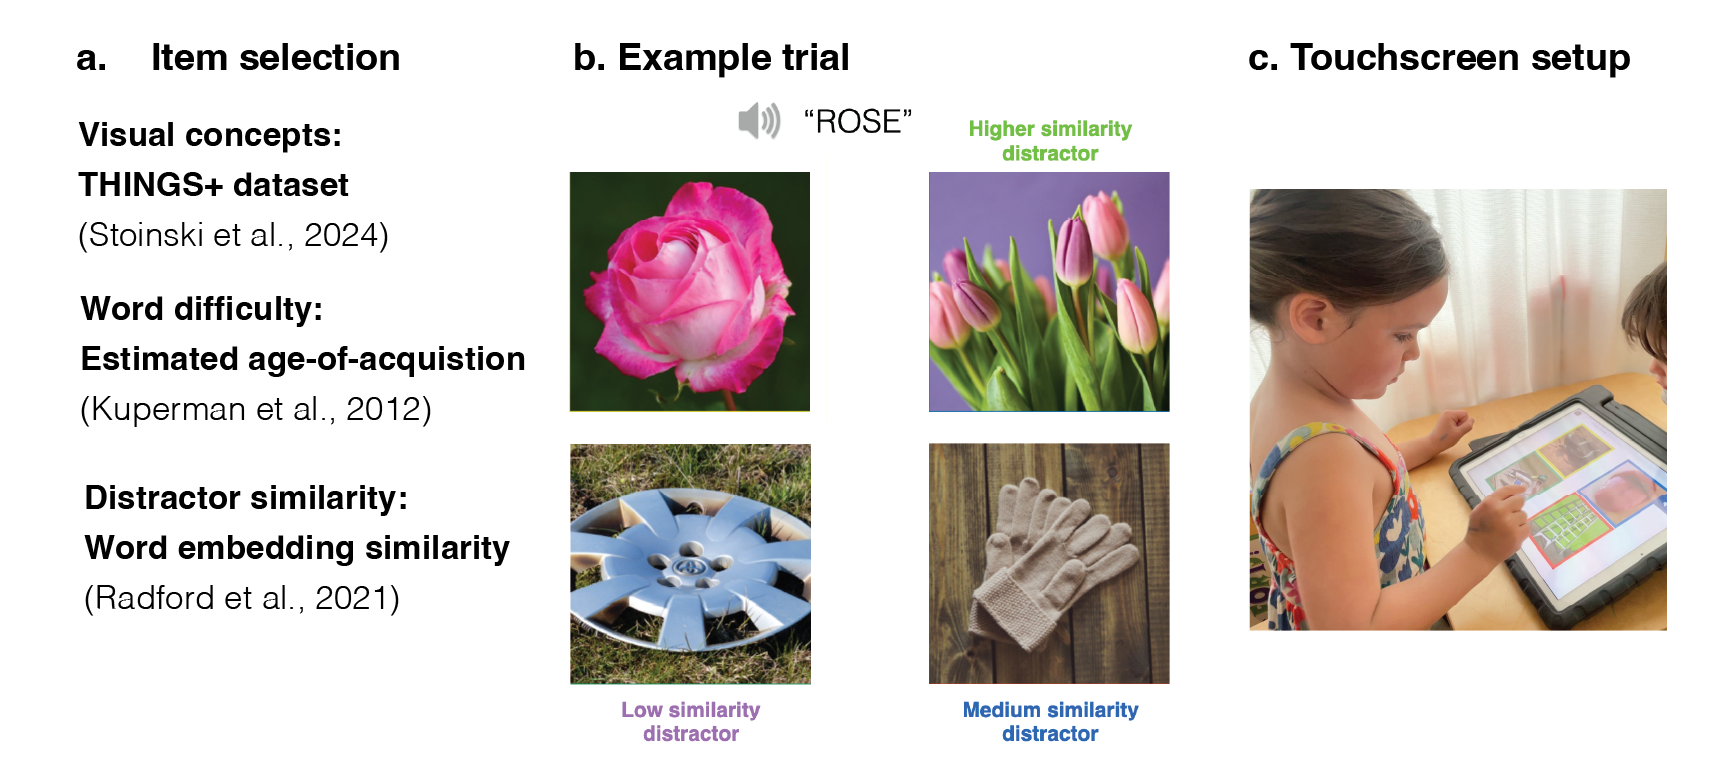
\includegraphics[width=1\linewidth]{visvocab-overview} 

}

\caption{Overview of the (a) databases and models involved in item selection, (b) an example trial, and (c) a touchscreen setup for younger participants. }\label{fig:procedure-figure}
\end{figure}

\subsection{Procedure}\label{procedure}

Children were invited to participate in a picture matching game where children were asked to help ``teach aliens on another planet about some of the words on our planet'' and children picked a particular alien to ``accompany them on their journey.'' Before the stimuli appeared, children heard a target word (e.g., ``apple'') and then were asked to ``choose the picture that goes with the word''. The four images appeared in randomized locations on the screen, and one of the images always corresponded to the target word (see example trial in Figure \ref{fig:procedure-figure}b). On practice trials, the distractor images were all very dissimilar to the target concept, and the target word was relatively easy. The tablet played a chime sound if children chose the correct image, and a slightly unpleasant sound if they responded incorrectly. Each child viewed a random subset of the item bank, and the items they viewed were displayed in a random order. Children were allowed to stop the game whenever they wanted to. Different versions of the game included varying amounts of trials or items; these games were developed as part of a project to develop an open-sourced measure of children's vocabulary knowledge. Here, we analyze children's responses to items that were generated using the THINGS+ dataset with distractors of varying difficulty (see Stimuli).

\subsection{Participants}\label{participants}

To obtain a large sample, we collected data from children in several different testing contexts. We collected data from children in an in-person preschools (\(N\) = 65, 3-5 year-olds), from the Children Helping Science Platform, (\(N\)=243, 3-7 year-olds), elementary schools across multiple states (\(N\)=3332, 5-14 year-olds) and adults online (\(N\)=211 adults, recruited via Prolific; half of the adults spoke English as a second language). Most participants responded directly via a keyboard, except those recruited online: however, children's parents responded via clicking on the image on Children Helping Science, and adults responded via clicking on the images.

We included data for a total of 3786 participants from preschools, schools, and online testing contexts around the United States (range 84 to 654), who completed, on average, 25.02 4AFC trials that were sampled randomly from the stimuli set (max = 86; different maximum numbers of trials were included in different testing contexts). All participants who contributed data and scored above 30\% accuracy were included, even if they did not complete the assessment (minimum trials = 2, maximum trials = 86, average number of trials = 25.02, We tested an additional 84 participants who scored near chance on 4AFC trials (chance = 25\%, threshold = 30\%) and were school-aged (\textgreater6 years of age) and who we excluded from analyses; these participants completed an average of 17.72 trials.

\subsection{Stimuli selection}\label{stimuli-selection}

We capitalized on publicly available existing image and audio databases to generate stimuli. Visual concepts were taken from the THINGS+ dataset (Stoinski et all., 2023), after filtering out non-child safe images (e.g., weapons, cigarettes) and images with low nameability (\textless.3), as per the released norming data. We used the copy-right free, high-quality image released for each visual concept. We then subset to visual concepts that had available audio recordings in the MALD database as well as age-of-acquisition (AoA) ratings from a previous existing dataset (Kuperman, 2012).

Using this subset, we sampled distractors with high, medium, and low similarity to the target word as operationalized via embedding similarity of the words in the language encode of a multimodal large language model (Radford et al., 2021).We determined high-, medium, and low similarity values relative to the distribution of all possible target-distractor pairing values for each word in the THINGS+ dataset. Stimuli were selected to optimize for having a maximum number of trials with unique target and distractors, in addition, we constrained the sampling such that target-distractor pairs had estimated age of acquisition within 3 years of each other. All stimuli and their meta-data are available on the public repository for this project. For each target word, we first selected a high-similarity distractor that had the highest cosine similarity to the target (and was itself not one of the target words). For medium-similarity distractors, we randomly sampled a distractor word was the same animacy as the target word, and unique to the dataset. For low-similarity words, we sampled a unique distractor words that had the lowest cosine similarity among the remaining distractors. In our final set, we had 108 items with a range of different estimated age-of-acquisitions (e.g., hedgehog, mandolin, mulch, swordfish, waterwheel, bobsled) with all unique targets and distractors. See Appendix, Figure XX for a visualization of the cosine similarity values for each distractor type for each word.

\subsection{Model features}\label{model-features}

We obtained all model features features using the Open AI available implementation of CLIP available at \url{https://github.com/openai/CLIP}. For language similarity, we computed the cosine similarity of the embeddings of the target word to each distractor word on each trial (e.g,. rose -- tulip, rose -- glove, rose -- hubcap). For visual similarity, we repeated this procedure but by obtaining image similarity vectors in the vision transformer for each target image and distractor image on each trial. For multimodal similarity, we computed the cosine similarity of the embedding of the target word in the language model to the embeddings for each of the distractor images; this is possible because the embedding spaces for the vision and language transformers in the CLIP model are aligned and have the same number of dimensions.

\subsection{Data and code sharing}\label{data-and-code-sharing}

These data were collected with the secondary goal of creating an open-source measure of children's developing vocabulary knowledge. These analyses presented in the paper were not pre-registered, and children's data were analyzed both during and at the end of data collection. All pre-processed data and analysis and plotting code have been made available in an online repository. The raw, trial-by-trial data cannot be shared due to data sharing agreements between the participating schools and the institution's IRB.

\section{Results}\label{results}

\begin{figure}[H]

{\centering \includegraphics[width=0.9\linewidth]{paper1_visualvocab_files/figure-latex/accuracy-fig-1} 

}

\caption{Visual vocabulary task performance as a function of the age of the child completing the task, plotted separately for relatively easy, harder, or difficult words; words are binned into terciles based on the estimated AoA from Kuperman et al., 2012. Lines refer to the proportion of words that children chose the target (red), high-similarity (green), medium similarity (turqouise), or low similarity (purple) distractor  at each age; error bars represent boostrapped confidence intervals.}\label{fig:accuracy-fig}
\end{figure}

\subsection{A protracted developmental trajectory}\label{a-protracted-developmental-trajectory}

We found a gradual increase in children's ability to correctly identify the target word across our entire age range, extending into early adolescence; Figure \ref{fig:accuracy-fig} shows the proportion of time that children identified the target word, highlighting a protracted developmental trajectory. We found this developmental trend for both relatively ``easy'' words, with an average estimated age-of-acquisition (AoA) of 4.81 years (SD = 0.87), more difficult words (average AoA =6.95 years, \(SD\) = 0.65 years), and challenging words (average AoA =9.60 years, \(SD\) = 1.21)).

At an item level, the words that showed the greatest change across age included some animals (e.g., ``swordfish'') as well as inanimate objects (``prism'',``antenna'',``sandbag'', ``turbine'') but also parts of larger buildings (``scaffolding'',``gutter''). However, some of our developmental trends likely also stem from differences in executive control: for some words that had very semantically similar distractors but were relatively easy (e.g., ``cheese'' vs ``butter''), we still saw steep developmental changes, highlighting that this ``simple'' picture vocabulary matching tasks still assess many different cognitive abilities beyond the fidelity of children's visual representations.

\subsection{Changes in the precision of visual concepts}\label{changes-in-the-precision-of-visual-concepts}

Next, we thus aimed to understand whether we were indeed observing changes in the precision of children's visual concepts. Indeed, one possibility is that children are mostly becoming more accurate at ignoring relevant distractors (due to developmental changes in executive function capacity), but often know what the target word refers to. If this is the case, then we should only observe changes how accurate children are at identifying the target word, with no changes in the types of distractors that children choose when they choose incorrectly. However, if children's visual concepts are proceeding from a coarse representations that is overly broad, or starting from no representation at all, then we would expect younger children to be more likely to choose distractors of all types, whereas we would expect older children to almost exclusively choose related distractors.

We thus examined whether we observed systematic changes in how children made errors across age, shown in Figure \ref{fig:errorbyage}. Consistent with the latter hypothesis, we found that children increasingly choose related distractors throughout development, with adults being still more likely to choose the related distractors relative to the oldest children (14-year-olds) in our sample.

\begin{table}
\centering
\caption{\label{tab:unnamed-chunk-21}Coefficients a linear regression  assessing changes in the proportion of related distractors chosen over development. Age and number of trials were standardized prior to analysis.}
\centering
\begin{tabular}[t]{lrrrr}
\toprule
Predictor & b & SE & t & p\\
\midrule
Intercept & 0.62 & 0.01 & 123.63 & < .001\\
Age (scaled) & 0.04 & 0.01 & 7.45 & < .001\\
Number of errors (scaled) & -0.05 & 0.01 & -8.23 & < .001\\
\bottomrule
\end{tabular}
\end{table}

We confirmed this result via a linear regression, modeling the proportion of errors that each children chose related distractors as our dependent variable as a function of children's age (in years); we also included the number of errors each child made as covariate as this varied widely by participant and age group. We found a main effect of age (see Table 1): older children were more likely to choose related distractors relative to unrelated distractors. We also modeled these effects at the item level in a linear mixed-effect model, with random intercepts for each item, finding a fixed effect of age (see SI), and thus the same pattern of effects. Children become more likely to choose related distractors across development, suggesting a progression where children gradually build detailed knowledge about the visual referents of many challenging words.

\begin{figure}[H]

{\centering \includegraphics[width=0.75\linewidth]{paper1_visualvocab_files/figure-latex/errorbyage-1} 

}

\caption{Changes in the proportion of errors chosen as a function of childrens age, where green lines reflected higher similarity distractors. Dot size represents the number of errors made by children in each age group. Error bars represent 95 percent bootrstrapped confidence intervals.}\label{fig:errorbyage}
\end{figure}

\subsection{Modeling changes in children's error patterns}\label{modeling-changes-in-childrens-error-patterns}

\pandocbounded{\includegraphics[keepaspectratio]{paper1_visualvocab_files/figure-latex/unnamed-chunk-25-1.pdf}}

\begin{figure}[H]

{\centering 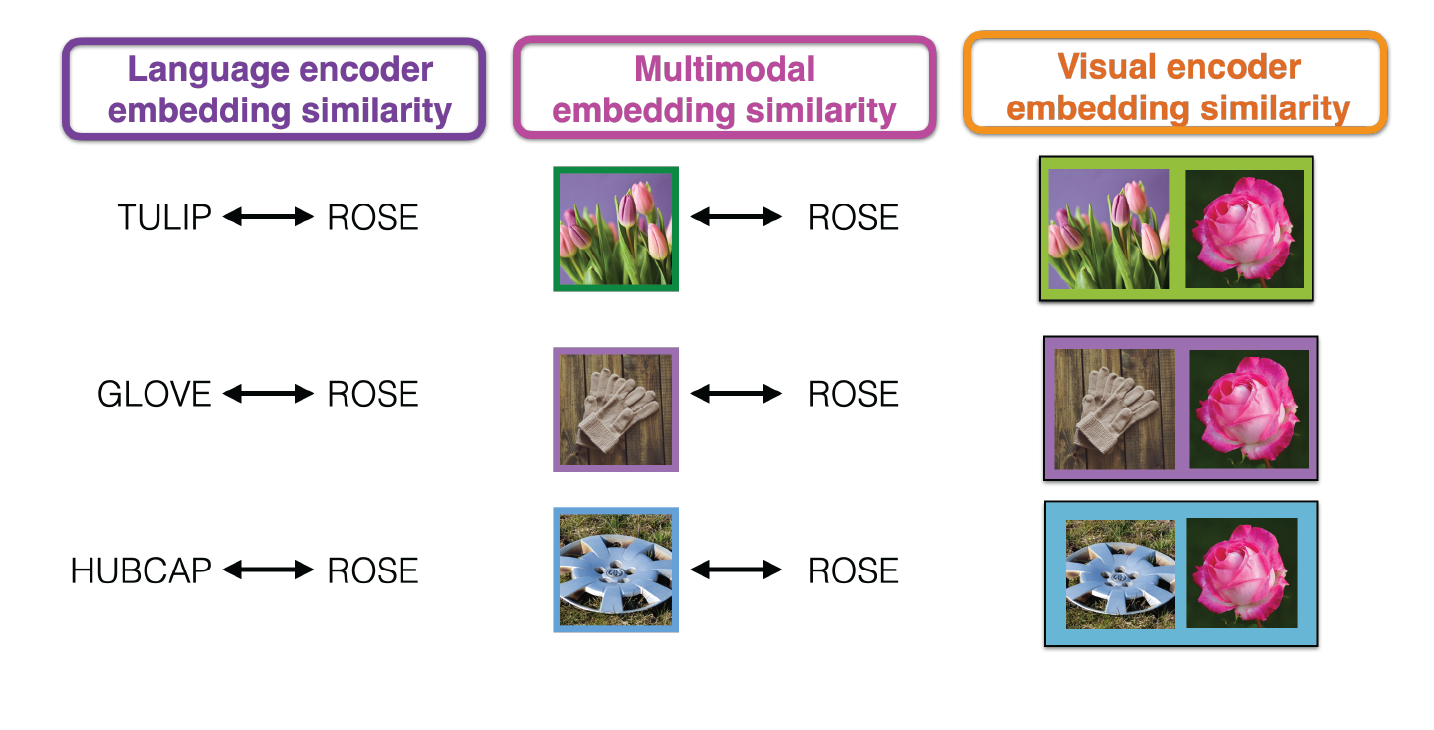
\includegraphics[width=1\linewidth]{embedding_similarity} 

}

\caption{Schematic of the three different ways that embedding simialrity was calculated in CLIP (Radford et al., 2021)}\label{fig:clip-figure}
\end{figure}

In a set of final analyses, we aimed to understand the source of these changes in children's error patterns by leveraging the high-dimensional embeddings of our linguistic and visual stimuli in the same large, multi-modal language model (Radford et al., 2021b) acknowledging that our stimuli were not necessarily designed to pull apart the contributions of changes in semantic versus visual similarity. Nonetheless, our stimuli were generated by using similarity in a linguistic embedding space, and so some stimuli on certain trials were nonetheless related to the target concept semantically but not necessarily visually (e.g, gardening ``gloves'' were a distractor for the target word ``rose''). We thus sought to understand the degree to which children's error patterns in this task reflected changes in how they processed the visual similarity of the targets and distractors, their semantic similarity, or--perhaps most likely--some combination.

To do so, we used a series of cross-validated linear mixed effect models, where we examined the degree to which visual, linguistic, and multimodal similarity metrics (and their combination) derived by large language model embeddings could explain children's error patterns. Specifically, we modeled the proportion of time that children chose each distractor for a target word as a function of the difficulty of the target word (as estimated by the estimated AoA metric), the age (in years) of the children participating, and (1) the similarity of the target word to each distractor word (linguistic embeddings), (2) the similarity of the target image to each distractor image (visual embeddings), and (3) the similarity of the target word to each distractor image (multi-modal embeddings), and (4) a combined model with all predictors combined. We iteratively sampled 80 percent of the dataset 50 times, and then evaluated the conditional R-squared for each model for each split; these values are plotted in Figure \ref{fig:modelfigure}. These exploratory results revealed that combining both the visual and linguistic embeddings -- either in one, large mixed-effect model, or via multi-modal embeddings -- led to increase explained variance in children's error patters. These results thus suggest that changes in children's error patterns across age are not solely due to changes in children's ability to reject the distractor images that are visually similar to the target concept.

\begin{figure}[H]

{\centering \includegraphics[width=0.5\linewidth]{paper1_visualvocab_files/figure-latex/modelfigure-1} 

}

\caption{Average explained variance in children's error patterns (conditional R-squared in linear mixed effect models) by linguistic, visual, multimodal, or combined predictors in cross-validated mixed efffect models. Error bars represent bootstrapped 95 percent confidence intervals across 50 iterations.}\label{fig:modelfigure}
\end{figure}

\begin{verbatim}
## <ScaleContinuousPosition>
##  Range:  
##  Limits: 0.15 --  0.3
\end{verbatim}

In a final analyses, we aimed to understand the source of these changes in children's error patterns by leveraging high-dimensional embeddings of our linguistic and visual stimuli in a large, multimodal language model (Radford et al., 2021b). We chose a set of stimuli where visual similarity was colinear with semantic similarity to a large degree, as it often is in the real-world for most visaul concepts. Thus, our stimuli were not necessarily designed to pull apart the contributions of changes in semantic vs.~visual similarity. Nonetheless, our stimuli were generated by using similarity in a linguistic embedding space, and so some stimuli on certain trials were nonetheless related to the target concept semantically but not necessarily visually (e.g, gardening gloves were a distractor for ``rose''). We thus sought to understand the degree to which children's error patterns in this task reflected changes in how they processed the visual similarity of the targets and distractors, their semantic similarity, or -- perhaps most likely -- some combination.

To do so, we used a series of cross-validated linear mixed effect models, where we examined the degree to which visual, linguistic, and multimodal similarity metrics (and their combination) derived by large language model embeddings could explain children's error patterns. Specifically, we modeled children's proportion of time that children chose each distractor for a target word as a function of the difficulty of the target word (as estimated by the estimated AoA metric), the age (in years) of the children participating, and (1) the similarity of the target word to each distractor word (linguistic embeddings), (2) the similarity of the target image to each distractor image (visual embeddings), and (3) the similarity of the target word to each distractor image (multi-modal embeddings), and (4) a combined model with all predictors combined. We iteratively sampled 80/\% of the dataset, and then evaluated the conditional r-squared for each model for each split; these values are plotted in Figure \ref{fig:modelfigure}. These exploratory results revealed that combining both the visual and linguistic embeddings -- either in one, large mixed-effect model, or via multi-modal embeddings -- led to increase explained variance in children's error patters. These results thus suggest that changes in children's error patterns across age are not solely due to changes in children's ability to reject the distractor images that are visually similar to the target concept.

\section{Discussion}\label{discussion}

How precise is children's visual concept knowledge, and how does this change across development? Here, we collect and analyze a large dataset of picture matching performance across development, finding evidence for a transition from coarse to finer-grained visual representations over early and middle childhood. Children became more accurate at identifying the referents of words over this entire age range, and their error patterns progressed from relatively random towards related distractors.

Broadly, these data support a theoretical view where these is substantial enrichment and change in existing representations for everyday visual concepts throughout childhood. For example, certain visual features may become more or less salient in children's visual concepts as children understand their functional roles (e.g., camels have humps to store water) or the degree to which they help delineate a category boundary (e.g., between whales and whale sharks). On this account, even school-aged children's visual representations may undergo substantial change as they learn more about the world around them.

This protraction of the timeline for visual concept learning into middle childhood substantially broadens the scope of potential learning mechanisms beyond associative label-object matching. For example, children's learning environments extend beyond the home and into structured educational contexts; children's learning partners include their peers, teachers, and siblings (who may be more or less reliable), and children's individualized experiences, interests, and hobbies may influence which words they have detailed visual representations for. As children begin to learn why animals and objects are classified the way they are, this semantic learning likely influences the visual features that are prioritized in children's representations. To make matters even more complicated, children also likely learn about visual features from generic utterances (e.g., ``Tigers have stripes'') (Gelman, Ware, \& Kleinberg, 2010) in verbal conversations where visual referents are nowhere to be found. Thus in order for our models and theories of visual concept learning to account for this full developmental trajectory, we need to think beyond labelled (or even captioned) photos or videos of referents.

Indeed, we suspect that visual concept learning extends into adulthood, and that many adults have coarse visual representations for many different words (and indeed, we culled some items during pilot testing because adults could not discriminate them!). Consider that while many adults in Western contexts experience the referents of some visual concepts relatively frequently e.g., trees, computers, cups, cars -- other words refer to visual concepts that different individuals may have varying amounts of interest in and frequency in interacting with -- like telescopes, or antelopes. Visual concept learning is likely influenced by both individuals pre-occupations and very intense interests, be they professional or not. And indeed decades of work has established that birding experts, car aficionados, (Tanaka \& Gauthier, 1997) and graphic artists (Perdreau \& Cavanagh, 2013) have both qualitatively and quantitatively different kinds of visual representations for the visual concepts that they engage with.

There are several limitations to the current work that future work could address. While we include data from a diverse group of children over a wide developmental age range, at present our conclusions are drawn primarily from around one hundred experimental items and distractors; further work that expands the range and diversity of the visual concepts -- and that expands to populations outside of the continental U.S.(Henrich, Heine, \& Norenzayan, 2010) will be necessary to understand the generalizability of these findings. In addition, the present data are large but cross-sectional, and thus cannot provide evidence for changes in the precision of representations within individual minds. Dense data collected from children over longer ranges of developmental time could confirm the hypotheses and theories raised by these analyses. Nonetheless, the present work highlights the promise of large-scale, online games for collecting large datasets that can be used to examine the consistency and variability in visual concept representations across childhood.

Overall, these findings suggest that children's visual concepts gradually become more precise across childhood, and broaden our view on the timeline and mechanisms for visual concept learning. We hope that future work will build on the tools and ideas developed here to understand the visual mind in both children and adults.

\newpage

\section{Acknowledgments}\label{acknowledgments}

This was was supported by a {[}BLINDED{]} to {[}BLINDED{]}. We gratefully acknowledge the children, families, and schools who participated in these studies, and members of the {[}BLINDED{]} and {[}BLINDED{]} labs who provided valuable feedback on the design of these studies. We also thank {[}BLINDED{]} for aiding with initial stimuli and task design.

\section{References}\label{references}

\phantomsection\label{refs}
\begin{CSLReferences}{1}{0}
\bibitem[\citeproctext]{ref-ayzenberg_development_2024}
Ayzenberg, V., \& Behrmann, M. (2024). Development of visual object recognition. \emph{Nature Reviews Psychology}, \emph{3}(2), 73--90. \url{https://doi.org/10.1038/s44159-023-00266-w}

\bibitem[\citeproctext]{ref-bergelson2017nature}
Bergelson, E., \& Aslin, R. N. (2017). Nature and origins of the lexicon in 6-mo-olds. \emph{Proceedings of the National Academy of Sciences}, \emph{114}(49), 12916--12921.

\bibitem[\citeproctext]{ref-bloom_how_2000}
Bloom, P. (2000). \emph{How children learn the meanings of words}. Boston, MA: MIT Press.

\bibitem[\citeproctext]{ref-braginsky_consistency_2019}
Braginsky, M., Yurovsky, D., Marchman, V. A., \& Frank, M. C. (2019). Consistency and variability in word learning across languages. \emph{Open Mind}, \emph{3}, 52--67. https://doi.org/\url{https://doi.org/10.1162/opmi_a_00026}

\bibitem[\citeproctext]{ref-dunn2003peabody}
Dunn, L. M., Dunn, D. M., \& Bulheller, S. (2003). \emph{Peabody picture vocabulary test: PPVT}. Swets Test Services.

\bibitem[\citeproctext]{ref-fernald2008looking}
Fernald, A. E., Zangl, R., Portillo, A. L., \& Marchman, V. A. (2008). Looking while listening: Using eye movements to monitor spoken language comprehension by infants and young children. In \emph{Developmental psycholinguistics: On-line methods in children's language processing} (pp. 97--135). John Benjamins Publishing Company.

\bibitem[\citeproctext]{ref-gelman2010effects}
Gelman, S. A., Ware, E. A., \& Kleinberg, F. (2010). Effects of generic language on category content and structure. \emph{Cognitive Psychology}, \emph{61}(3), 273--301.

\bibitem[\citeproctext]{ref-gershon2014language}
Gershon, R. C., Cook, K. F., Mungas, D., Manly, J. J., Slotkin, J., Beaumont, J. L., \& Weintraub, S. (2014). Language measures of the NIH toolbox cognition battery. \emph{Journal of the International Neuropsychological Society}, \emph{20}(6), 642--651.

\bibitem[\citeproctext]{ref-henrich2010most}
Henrich, J., Heine, S. J., \& Norenzayan, A. (2010). Most people are not WEIRD. \emph{Nature}, \emph{466}(7302), 29--29.

\bibitem[\citeproctext]{ref-long2024parallel}
Long, B., Fan, J. E., Huey, H., Chai, Z., \& Frank, M. C. (2024). Parallel developmental changes in children's production and recognition of line drawings of visual concepts. \emph{Nature Communications}, \emph{15}(1), 1191.

\bibitem[\citeproctext]{ref-perdreau2013artists}
Perdreau, F., \& Cavanagh, P. (2013). Is artists' perception more veridical? \emph{Frontiers in Neuroscience}, \emph{7}, 6.

\bibitem[\citeproctext]{ref-pereira2009developmental}
Pereira, A. F., \& Smith, L. B. (2009). Developmental changes in visual object recognition between 18 and 24 months of age. \emph{Developmental Science}, \emph{12}(1), 67--80.

\bibitem[\citeproctext]{ref-radford_learning_2021}
Radford, A., Kim, J. W., Hallacy, C., Ramesh, A., Goh, G., Agarwal, S., et al.others. (2021b). Learning transferable visual models from natural language supervision. \emph{International Conference on Machine Learning}, 8748--8763. PMLR.

\bibitem[\citeproctext]{ref-radford2021learning}
Radford, A., Kim, J. W., Hallacy, C., Ramesh, A., Goh, G., Agarwal, S., et al.others. (2021a). Learning transferable visual models from natural language supervision. \emph{International Conference on Machine Learning}, 8748--8763. PmLR.

\bibitem[\citeproctext]{ref-rosch1978principles}
Rosch, E. (1978). \emph{Principles of categorization}.

\bibitem[\citeproctext]{ref-suggate2018infancy}
Suggate, S., Schaughency, E., McAnally, H., \& Reese, E. (2018). From infancy to adolescence: The longitudinal links between vocabulary, early literacy skills, oral narrative, and reading comprehension. \emph{Cognitive Development}, \emph{47}, 82--95.

\bibitem[\citeproctext]{ref-tanaka1997expertise}
Tanaka, J., \& Gauthier, I. (1997). Expertise in object and face recognition. \emph{Psychology of Learning and Motivation}, \emph{36}, 85--126.

\bibitem[\citeproctext]{ref-vales_lumping_2020}
Vales, C., Stevens, P., \& Fisher, A. V. (2020). Lumping and splitting: {Developmental} changes in the structure of children's semantic networks. \emph{Journal of Experimental Child Psychology}, \emph{199}, 104914.

\bibitem[\citeproctext]{ref-waxman2009early}
Waxman, S. R., \& Gelman, S. A. (2009). Early word-learning entails reference, not merely associations. \emph{Trends in Cognitive Sciences}, \emph{13}(6), 258--263.

\bibitem[\citeproctext]{ref-weaver2024becoming}
Weaver, H., Zettersten, M., \& Saffran, J. R. (2024). Becoming word meaning experts: Infants' processing of familiar words in the context of typical and atypical exemplars. \emph{Child Development}, \emph{95}(5), e352--e372.

\end{CSLReferences}


\clearpage
\renewcommand{\listfigurename}{Figure captions}


\end{document}
